% ── 1. Introduction ───────────────────────────────────────────────────────────
\section{Introduction}

Hearing aids face a fundamental challenge in multi-talker environments: the cocktail party problem. Even for normal-hearing listeners, selectively attending to one speaker among many is demanding — for hearing aid users it is significantly harder. The small form factor of a behind-the-ear device imposes strict limits on spatial resolution, and the user cannot simply turn their head to a preferred speaker the way a sighted person might orient their gaze.

For this case, I analyse a four-channel hearing aid recording containing seven simultaneous speakers. I identify and name each talker, estimate their directions of arrival, produce full transcriptions, determine the most likely talker of interest, and deliver an enhanced audio signal isolating that target speaker.

% ── 2. Validation on Example Mixture ─────────────────────────────────────────
\section{Validation on Example Mixture}

\subsection{Microphone Array Geometry}

The hearing aid is a behind-the-ear (BTE) device with four microphones: two on the left ear and two on the right. The inter-ear baseline — the distance across the head — is approximately 16\,cm, giving a maximum inter-ear time difference of around 0.47\,ms (21.5 samples at 44.1\,kHz). Each intra-ear microphone pair is separated by roughly 8\,mm (front and rear ports on the same ear unit). Channels are ordered left-front, left-rear, right-front, right-rear.

The short intra-ear baseline has a fundamental consequence for front/rear disambiguation. A source at 0° (front) and one at 180° (back) produce inter-aural time differences of equal magnitude but opposite sign — yet for the intra-ear pair the TDOA difference is less than 2 samples. Parabolic interpolation of the GCC-PHAT peak cannot reliably resolve differences this small in a noisy mixture, so front and rear sources are effectively ambiguous from geometry alone. This ambiguity persists throughout the analysis and is acknowledged where relevant.

% Figure: array diagram (from case PDF)

\subsection{Comparison Tool}

To evaluate separation results rapidly and systematically, I built an interactive HTML player (\texttt{demo/player.html}). The page loads a configurable list of audio tracks, presents them in grouped sections, and allows instant A/B switching between any two sources with a single click. All BSS output variants, isolation passes, noise reduction sweeps, and raw mixture channels are accessible in one place without switching tools or writing scripts. This made it straightforward to judge the perceptual quality of each parameter choice during the Optuna search and to confirm speaker identities by listening while reading the transcripts side-by-side.

% Figure: demo screenshot

\subsection{SRP-PHAT}

As a first spatial analysis step I ran SRP-PHAT — a broadband beamformer that scans a grid of candidate directions and accumulates generalised cross-correlation (PHAT-weighted) energy for each pair of microphones. For the example mixture, whose four speaker positions were given in the case materials, the azimuth peaks recovered by SRP-PHAT matched the known positions to within a few degrees for the two strongly lateral sources. Near-frontal and near-rear sources produced peaks near 0°/180° as expected, though front/rear discrimination remained unreliable for the reasons described above. This validated the pipeline before applying it to the main mixture, where ground-truth positions are unknown.

\subsection{FastMNMF2 and Bayesian Optimisation}

FastMNMF2 \cite{} is a multichannel non-negative matrix factorisation algorithm that estimates independent source spectrograms and full-rank spatial covariance matrices jointly. Applied to the example mixture with $n{=}4$ sources, it produced clean separations of all four speakers. One pair of sources was labelled front/rear in the reverse order from the ground truth — consistent with the geometric ambiguity above — but the audio content was correct.

To maximise separation quality on the main mixture I used Optuna \cite{} to search over STFT frame size (512–4096), hop fraction (0.25–0.5), number of EM iterations (30–200), and number of NMF components per source (2–16). The objective was the sum of pairwise cross-correlation magnitudes across source pairs — lower values indicate more independent outputs. Sixty trials were run on the DTU HPC cluster (8 CPU cores, 32\,GB RAM, 24-hour wall time).

% ── 3. Mixture Analysis ───────────────────────────────────────────────────────
\section{Mixture Analysis}

\subsection{Speaker Identification}

Running repeated BSS sweeps with varying initialisation revealed seven distinct voices in the mixture. I named each speaker after a salient topic in their speech for ease of reference: \textit{Convo Man} and \textit{Convo Woman} (a couple having a conversation), \textit{Australia Man}, \textit{Birthday Brunch Woman}, \textit{Mountain Man}, \textit{Ageing Man}, and \textit{Burning House Man}. Full transcriptions produced by careful listening are given in Appendix~\ref{sec:transcripts}.

\subsection{Initial DoA Estimation}

A quick initial DoA estimate came from listening to the raw left and right channels in isolation. Australia Man was immediately identifiable as strongly left-dominant: his voice was clearly louder in channel 1 (left-front) than in channel 3 (right-front). Conversely, Birthday Brunch Woman was right-dominant. The two lateral speakers were therefore identified and their approximate azimuths — $\sim$90° and $\sim$270° respectively — were confirmed before any algorithmic processing.

\subsection{Inter-Ear Spectro-Temporal Binary Masking}

To suppress the strongly lateral sources and expose the remaining five near-axis speakers, I applied an inter-ear spectro-temporal binary mask. For each time-frequency bin I computed the ratio of left-channel to total power:
\[
  r(t,f) = \frac{|X_L(t,f)|^2}{|X_L(t,f)|^2 + |X_R(t,f)|^2}
\]
Bins where $r < 0.35$ (right-dominated) or $r > 0.65$ (left-dominated) were zeroed across all four channels; only bins within the central 30\% of the ratio range were passed. This retained 15.7\% of all TF bins — the subset dominated by near-midline sources — and substantially reduced the energy contribution of Australia Man and Brunch Woman in subsequent BSS passes.

\subsection{Activity-Weighted SRP-PHAT}

With a clean BSS isolation of each speaker I could steer the SRP-PHAT accumulation to frames where that speaker is active, rather than integrating over the full mixture. For each source I computed per-frame RMS energy and retained the top 15\% most-active frames as a binary activity mask. SRP-PHAT was then accumulated across the four raw channels using only those frames.

For the two lateral speakers the raw mixture was used directly; for the five near-axis speakers the inter-ear masked mixture was used to prevent Australia Man and Brunch Woman from dominating the spatial histogram even during frames where they are quiet. After identifying the primary peak, a second peak was located after suppressing a $\pm$15° window around the first, providing a confidence measure: a strong second peak at $+$180° from the first indicates front/rear ambiguity rather than a genuine second source. Results are summarised in Table~\ref{tab:results}.

\subsection{Talker of Interest}

Convo Woman was markedly louder than every other speaker across the entire recording — her energy in the BSS output exceeded all others by a consistent margin. The most natural explanation is that she is the closest source to the microphone array, i.e.\ the hearing aid wearer herself. Her activity-weighted DoA scan places her at $\sim$180° or 0° — the same front/rear ambiguity as the other near-axis speakers, consistent with a source directly on the listener's axis.

Convo Man is her direct conversational partner: he responds turn-by-turn, his pauses align with her speech, and the content of the exchange is a coherent back-and-forth. His estimated DoA places him at $\sim$0° or 180° — consistent with directly in front of the listener, the natural position for a face-to-face conversation. Five of the remaining six speakers are delivering monologues with no interlocutor present, making Convo Man the only external source with a clear social relationship to the wearer. He is therefore the talker of interest.

% ── 4. Target Enhancement ─────────────────────────────────────────────────────
\section{Target Enhancement}

FastMNMF2 with $n{=}4$ sources was applied to the inter-ear masked four-channel signal. With the strongly lateral sources suppressed, source 3 of the Optuna-optimised run consistently captured Convo Man with minimal cross-talk from the remaining speakers.

Post-separation, spectral noise reduction was applied using the \texttt{noisereduce} library in non-stationary mode with a noise power reduction factor of 0.8. This setting was selected after a blind listening sweep of ten variants (stationary vs.\ non-stationary noise models, reduction factors 0.8–1.0, Wiener filtering, and bandpass-only approaches): non-stationary with $\text{prop}=0.8$ best preserved the natural timbre of the voice while suppressing the residual diffuse background. The final output is \texttt{target\_speaker\_enhanced.wav}.

% ── 5. Results ────────────────────────────────────────────────────────────────
\section{Results}

\begin{table}[H]
\centering
\caption{Identified speakers with estimated DoA and gender.}
\label{tab:results}
\begin{tabular}{llll}
\toprule
\textbf{Speaker} & \textbf{Gender} & \textbf{Est.\ DoA} & \textbf{Notes} \\
\midrule
Convo Man         & M & $\sim$0° (front)   & \textbf{Talker of interest} \\
Convo Woman       & F & $\sim$0° or 180°   & Likely wearer; front/rear ambiguous \\
Australia Man     & M & $\sim$90° (left)   & Confirmed \\
Brunch Woman      & F & $\sim$270° (right) & Confirmed \\
Mountain Man      & M & $\sim$0° (front)   & Strong confidence \\
Ageing Man        & M & $\sim$180° (back)  & Moderate confidence \\
Burning House Man & M & $\sim$180° (back)  & Estimated \\
\bottomrule
\end{tabular}
\end{table}

\subsection{Microphone Selection}

FastMNMF2 estimates a full-rank $4\times4$ spatial covariance matrix for each source, and the separated output is reconstructed as a weighted combination of all four input channels. This is preferable to selecting a single microphone: a near-frontal source that is roughly equidistant from all four capsules benefits from coherent averaging across the array, which suppresses spatially diffuse noise without the directional nulling artefacts that a fixed beamformer would introduce for a source near its steering axis.

The enhanced output is delivered as \texttt{target\_speaker\_enhanced.wav}.

% ── 6. Going Further ──────────────────────────────────────────────────────────
\section{Going Further}

The most promising extension would be to fine-tune a supervised separation model — such as SepFormer or TF-GridNet — on a synthetic dataset matched to the seven-speaker scenario. I generated a Libri7Mix dataset using the LibriMix pipeline, simulating seven-speaker mixtures from LibriSpeech utterances convolved with randomised room impulse responses. The data generation pipeline ran on the DTU HPC cluster (A100 GPU node), but a storage quota approval came too late for training to complete before the deadline. With sufficient compute and storage this approach would likely outperform the unsupervised BSS methods used here, particularly for front/rear disambiguation and for sources with overlapping spectral content.

% ── Appendix ──────────────────────────────────────────────────────────────────
\appendix
\section{Case Description}
\label{app:case}
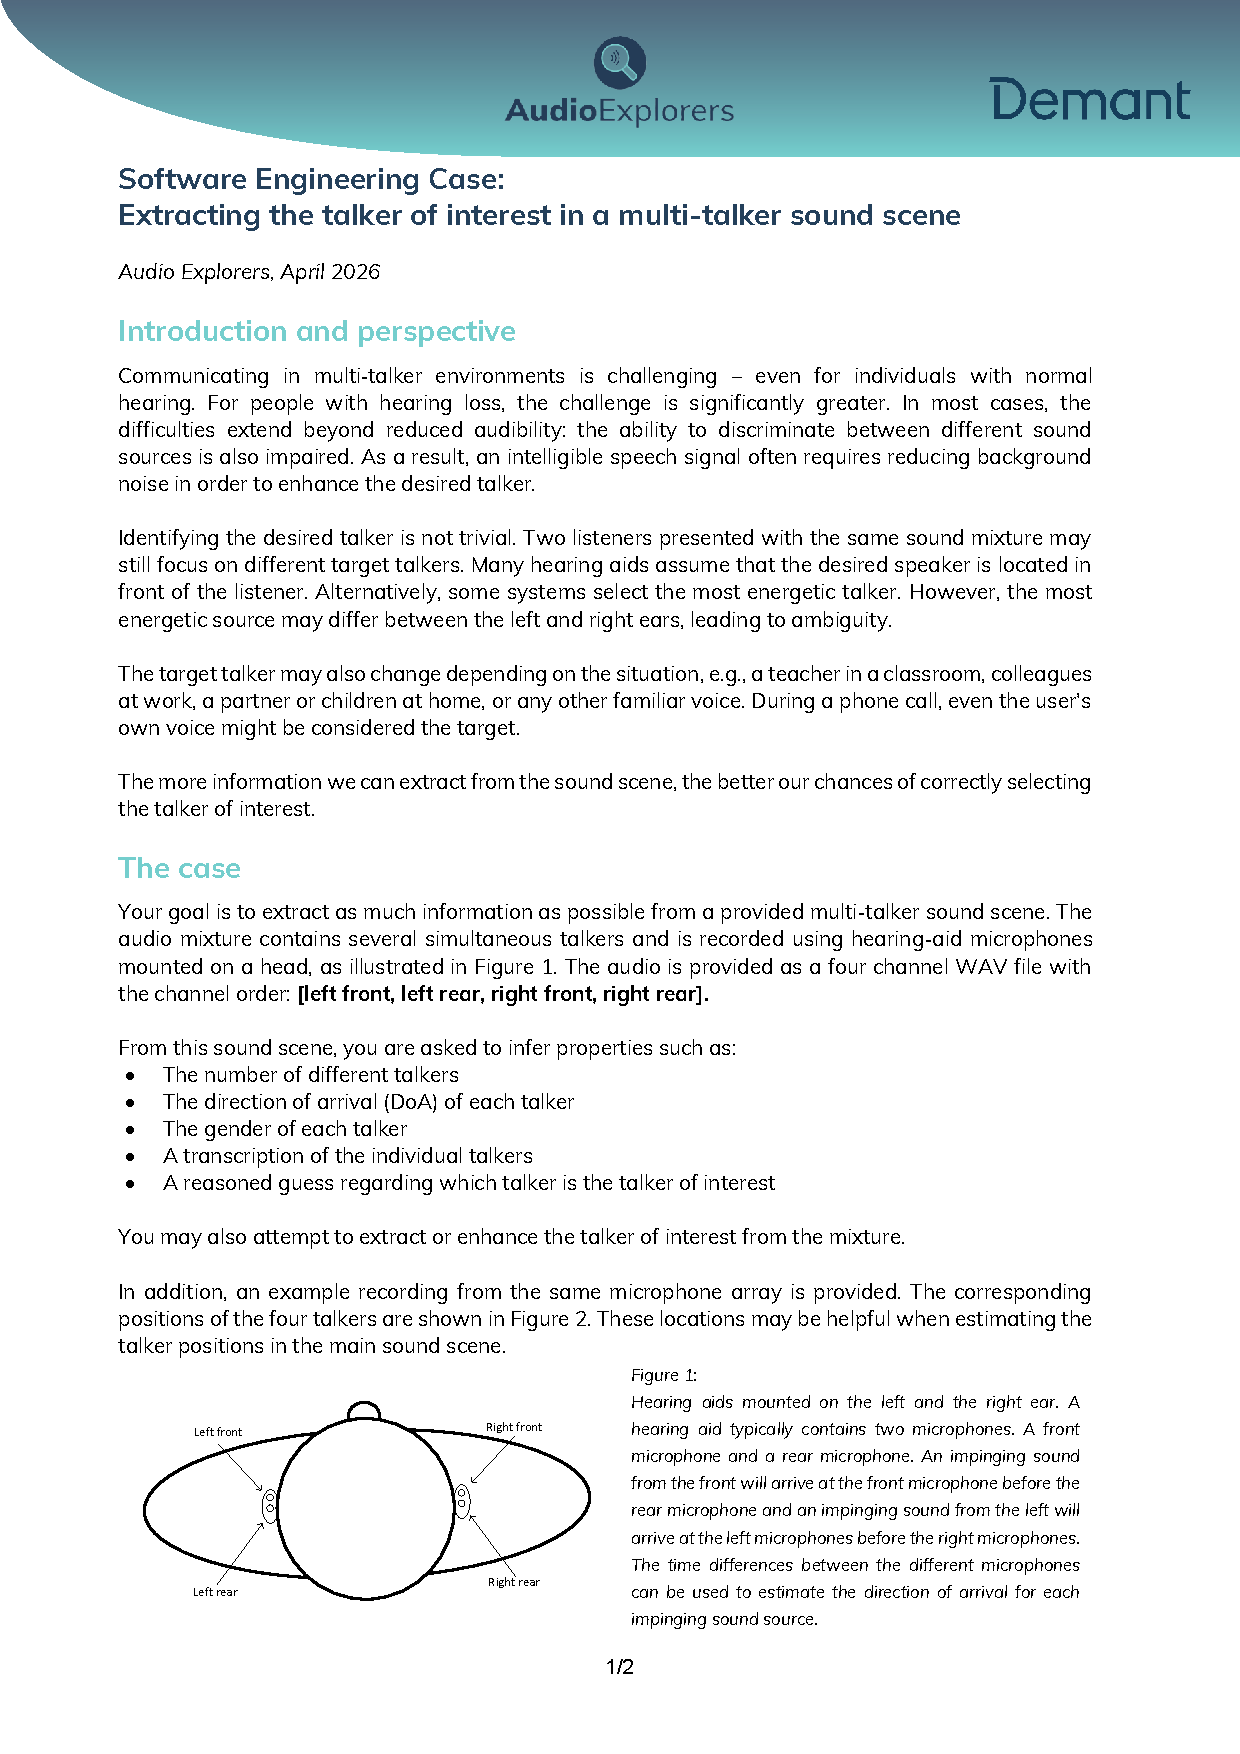
\includepdf[pages=-]{../case.pdf}

\section{Full Transcripts}
\label{sec:transcripts}

\subsection*{Convo Couple}
\textbf{M:} Hi, how are you? \textbf{W:} Great, how are you? \textbf{M:} I just had my birthday. \textbf{W:} Really, how old are you? \textbf{M:} I am 35. \textbf{W:} Are you married? \textbf{M:} Yes, I got married 3 years ago. \textbf{W:} Do you have any children? \textbf{M:} Yes, I have a daughter. She is 4 years old. Do you have children? \textbf{W:} Yes, I have two. My older son is 5, and my younger son is 3.

\subsection*{Australia Man}
Most sightseers will be Chinese, and for the great majority, this 83 million monument to life down under was the closest they'll come to visiting Australia. Australia's Commissioner-General to Expo, Lyndall Sachs, says: ``There's a lack of knowledge here about Australia. They just think we blow stuff up out of the earth and export it.''

\subsection*{Birthday Brunch Woman}
Every year at my birthday brunch, guests elbow each other over the smoked salmon, while a bowl of pickled herring sits forlornly, mostly untouched. I should probably stop buying it, but I like it, and it's my birthday, after all. This year was no exception, and at the end---

\subsection*{Mountain Man}
I had never thought about climbing Kilimanjaro until I learned of its statistics. Over 25,000 climbers attack it each year, 40\% can't make it to the top, and a handful don't make it down at all. A foolish curiosity set in --- might be a winner, or a loser.

\subsection*{Ageing Man}
It is inevitable: the muscles weaken, hearing and vision fade, we get wrinkled and stooped, we can't eat, run or even walk as fast as we used to. We have aches and pains of our body never noticed before. We get old. It sounds miserable, but apparently, it's not. A large Gallup poll found that by almost any measure,~---

\subsection*{Burning House Man}
What would you save if your house was burning down? If a fire hit my house, I think I'd have this terrible guilt trip. I'd be running around picking up all the things that I haven't done. This teddy bear is not actually that special. I'd just feel really bad about having to exit. I've had it since I---
